%%
% BIThesis 本科毕业设计论文模板 —— 使用 XeLaTeX 编译 The BIThesis Template for Undergraduate Thesis
% This file has no copyright assigned and is placed in the Public Domain.
%%

\chapter{系统实现与测试}

\section{开发环境搭建}

\subsection{选择的技术栈}

本系统涉及移动客户端、服务端、管理后台端三个独立子项目，各端技术选型如下。

\begin{itemize}
  \item 移动客户端：Flutter 3.41.9 + Dart，使用 GetX 进行状态管理与路由控制
  \item 服务端：Rust 1.95.0 + Salvo Web 框架，通过 SQLx 连接 PostgreSQL
  \item 管理后台端：Vue 3 + TypeScript，使用 Element Plus 组件库与 Axios
  \item 接口契约：OpenAPI 3.0 规范文件，作为三端共享的接口定义基准
  \item 数据库：PostgreSQL 18.3
  \item 版本控制：Git 2.54.0
\end{itemize}

\subsection{软件环境配置}

\begin{itemize}
  \item 操作系统：Windows 11 + WSL2 (Ubuntu)
  \item 移动客户端开发：Flutter SDK 3.41.9
  \item 服务端开发：Rust 工具链 1.95.0（rustc、Cargo、Clippy）
  \item 管理后台端开发：Node.js 26.1.0
  \item 数据库：PostgreSQL 18.3 
  \item 版本控制：Git 2.54.0
  \item API 文档工具：Swagger UI 4.15.5
  \item IDE：Visual Studio Code 
\end{itemize}

\section{开发过程}

本系统的开发过程划分为以下四个阶段。

\begin{enumerate}
  \item 准备阶段
  \begin{itemize}
    \item 需求分析与功能边界确定
    \item 三端工程骨架搭建与编译环境配置
    \item 技术选型验证与原型页面开发
    \item OpenAPI 规范文件建立，作为开发与联调基准
  \end{itemize}

  \item 核心功能开发阶段
  \begin{itemize}
    \item 移动客户端：认证流程、课程浏览与章节阅读、代码编辑与提交评测、闯关挑战与每日任务、好友系统与排行榜
    \item 服务端：认证鉴权、课程内容提供、提交记录与评测、挑战状态管理、奖励结算、社交数据处理
    \item 管理后台端：课程管理、挑战管理、题目管理、用户管理、公告与运营配置
    \item 三端协同：通过 OpenAPI 工具链保持接口定义一致，变更后同步更新契约文件
  \end{itemize}

  \item 完善优化阶段
  \begin{itemize}
    \item 移动客户端：错误提示优化、离线状态感知、本地草稿保存、屏幕适配测试
    \item 服务端：错误分类与响应结构完善、异常容错、请求日志记录
    \item 管理后台端：表单交互优化、数据展示调整
  \end{itemize}

  \item 测试发布阶段
  \begin{itemize}
    \item 契约验证：基于 OpenAPI 文档进行 Schema 校验与示例对照
    \item 服务端功能测试：覆盖核心接口的功能正确性
    \item 跨端联调：验证管理后台端操作对移动客户端的可见性
    \item 项目文档整理与代码仓库交付
  \end{itemize}
\end{enumerate}

\section{移动客户端模块实现}

移动客户端以 Flutter 为运行容器、GetX 为状态管理与路由控制框架，整体遵循 View—Controller—Service 三层架构。每个页面由三个类组成——View 类负责界面渲染，Controller 类负责业务逻辑与状态管理，Binding 类负责依赖注入绑定——三者组织在同一个文件中，既保证了代码内聚性，又降低了页面间的耦合度。

\subsection{应用基础设施设计}

在应用入口实现上，系统通过屏幕适配工具处理不同尺寸设备上的界面缩放，并在初始化阶段依次完成推送服务、本地存储与全局依赖注入等准备工作。系统主程序采用统一的路由管理、主题控制、绑定注册与页面切换机制，同时在应用外层增加离线感知壳层，用于在网络不可用时提示用户学习记录将暂存本地。这种将基础服务准备放在用户可见界面之前的初始化顺序，有助于减少运行期异常对用户体验的直接影响。

所有页面 Controller 继承自统一的基类，基类封装了覆盖初始、加载中、空数据、错误、离线、认证过期和部分数据七种状态的通用状态机。每个页面的 View 层通过状态容器组件根据当前状态自动切换展示内容，避免在每个页面中重复编写状态判断逻辑，实现了状态处理逻辑的集中管理与复用。

全局服务通过依赖注入在应用启动时注册。网络服务层对 HTTP 客户端进行统一封装，集中处理基础地址、超时控制、认证令牌注入与错误拦截逻辑。当接口返回未授权状态时，网络层能够自动清除本地会话并引导跳转至登录页。本地存储服务封装了键值读写能力，用于持久化认证信息与用户偏好。进度服务作为核心离线引擎，维护章节完成、课程进度、挑战通关、奖励发放、每日挑战记录与待同步动作等学习状态。该服务将学习状态分为即时状态（用于界面渲染）与待处理状态（用于网络恢复后的后续处理）两类，并在网络状态监听触发时自动处理离线期间积累的待同步队列，从而提高弱网环境下学习行为记录的连续性。

移动客户端中所有 Controller 均采用 GetX 响应式状态管理模式，通过可观察对象驱动界面更新。以下示例展示了 Controller 的典型结构：以响应式列表管理数据集合，通过标记位控制加载和错误状态，并在初始化时自动触发数据获取。

\begin{lstlisting}[language=Dart, caption={GetX 响应式控制器示例}, label={lst:getx-controller}]
class ItemListController extends GetxController {
  final items = <Item>[].obs;
  final isLoading = false.obs;
  final error = Rxn<String>();

  @override
  void onInit() {
    super.onInit();
    fetchItems();
  }

  Future<void> fetchItems() async {
    isLoading.value = true;
    try {
      final res = await apiService.getItems();
      items.assignAll(res.data);
    } catch (e) {
      error.value = e.toString();
    } finally {
      isLoading.value = false;
    }
  }
}
\end{lstlisting}

\subsection{账户管理模块}

账户管理模块涵盖启动引导、登录注册与个人资料维护功能。启动阶段系统首先检查本地存储中的认证令牌，根据令牌有效性和首次使用状态决定进入主页、新手引导或登录页。

登录页面采用邮箱与密码表单，Controller 在表单验证通过后调用服务端认证接口，成功后持久化令牌并跳转至主页。注册页面在此基础上增加昵称与确认密码字段，完成注册后自动登录。新手引导以多步滑动页面的形式向学习者介绍学习、奖励、社交与进度四大核心功能。登录界面效果如图\ref{fig:mobile-login}所示。

\begin{figure}[htbp]
  \centering
  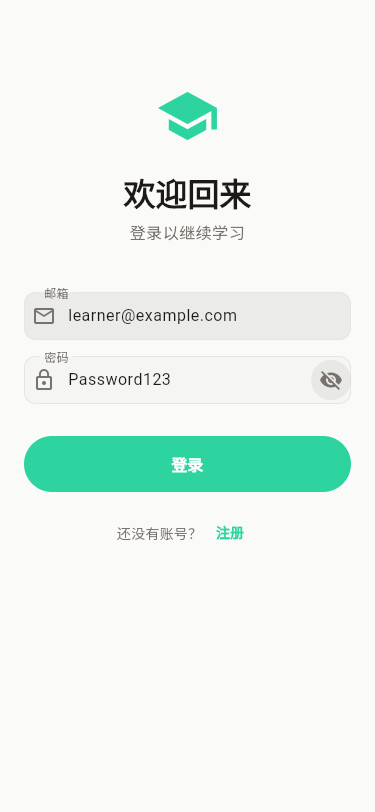
\includegraphics[width=0.35\textwidth]{images/mobile-login.png}
  \caption{移动客户端登录界面}
  \label{fig:mobile-login}
\end{figure}

登录后的个人资料编辑页面支持修改昵称、简介、每日学习目标与主题模式，通过服务端用户资料接口提交更新。设置页面提供账户信息查看、学习进度清除、主题切换、缓存管理、通知设置与退出登录等功能。退出登录时系统清除本地认证数据并将页面重置至登录页。

\subsection{课程学习模块}

课程学习模块是移动客户端的内容承载核心，包含课程列表、课程详情和章节阅读三个主要页面。

课程列表页面通过 Controller 获取课程数据，以列表形式呈现每门课程的封面、标题、简介与学习进度。该页面支持按难度、分类和完成状态三个维度进行筛选，同时提供关键词搜索功能，帮助学习者快速定位目标课程。筛选逻辑在客户端以响应式计算的方式实现，无需额外网络请求即可在已加载数据中切换视图。首页与课程列表效果如\ref{fig:mobile-home}所示。

\begin{figure}[htbp]
  \centering
  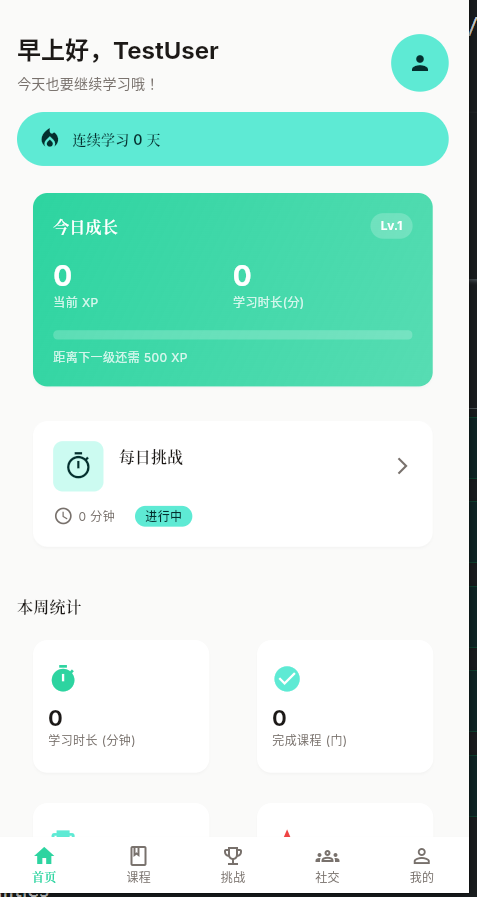
\includegraphics[width=0.35\textwidth]{images/首页.png}
  \caption{移动客户端首页与课程列表}
  \label{fig:mobile-home}
\end{figure}

课程详情页面采用可折叠式顶部区域展示课程封面与简介，下方以时间线形式排列章节列表。每个章节节点显示完成状态。系统通过链式锁定机制控制学习路径：若前置章节未完成，后续章节自动标记为锁定状态，点击时弹出提示弹窗而非直接进入，以此引导学习者按照设计好的知识递进顺序进行学习。课程的整体进度百分比根据已完成章节数动态计算。

章节阅读页面是知识内容的核心消费载体。页面以 Markdown 渲染器展示结构化教学内容，内嵌高亮的示例代码卡片与知识点总结面板。页面底部固定操作栏提供标记完成、返回课程或进入对应练习三个入口。完成操作后，进度服务记录章节完成状态、累加经验值，并检查是否为课程最后一个章节以触发课程完成奖励。章节阅读页面效果如图\ref{fig:mobile-reading}所示。

\begin{figure}[htbp]
  \centering
  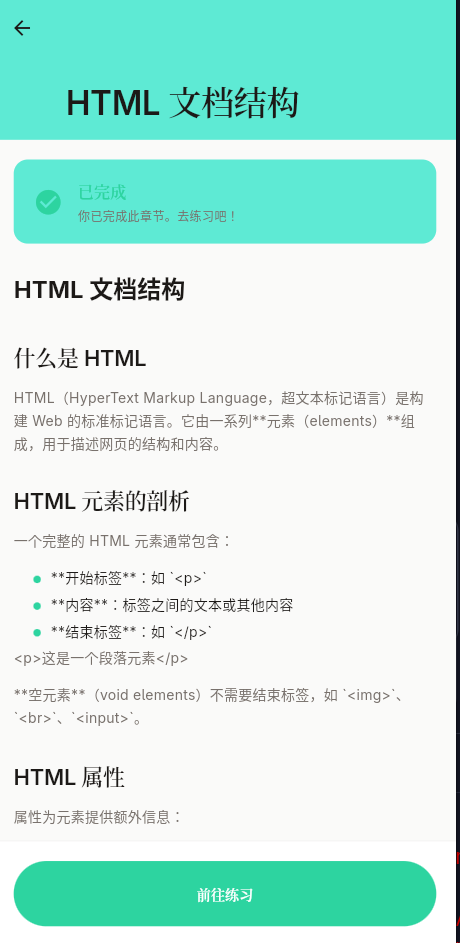
\includegraphics[width=0.28\textwidth]{images/章节阅读.png}
  \caption{移动客户端章节阅读页面}
  \label{fig:mobile-reading}
\end{figure}

离线场景下，课程列表与章节内容均通过本地缓存机制提供。服务端返回的课程数据在渲染前会与本地进度记录合并，使得离线状态下的进度展示仍然准确，保证学习者在弱网环境中的学习体验连续性。

\subsection{编码练习模块}

编码练习模块是学习闭环中“知识内化”的关键环节。练习页面的设计核心在于如何在移动设备有限的屏幕空间内同时承载题目描述、代码编辑区和结果反馈区。系统通过多标签页的工作区划分来解决这一矛盾：将代码编辑、实时预览和运行检查三个功能分别放置于独立标签页中，学习者通过切换标签页在不同操作阶段聚焦于当前任务。

代码编辑区配备了草稿自动保存机制：每次代码变更后经过防抖延迟，自动将当前代码保存至本地存储。当学习者离开页面后再次进入时，系统自动恢复上次编辑的草稿，避免因意外退出导致编辑内容丢失。

提交操作通过服务端评测接口完成。服务端返回的评测结果以底部弹窗形式呈现，包含分数、通过用例数、总用例数和结构化的反馈信息。对于首次提交即失败的场景，弹窗底部提示学习者可使用 AI 帮助功能；对于多次尝试后仍未通过的场景，弹窗给出更具引导性的建议。

\subsection{挑战系统模块}

挑战系统模块是游戏化学习机制的核心，包含闯关挑战与每日挑战两类挑战形式。

闯关挑战列表以可视化地图形式呈现。每个挑战节点按序号排列并通过连线连接，节点的视觉状态通过链式解锁逻辑推导：只有当前置节点完成后，后续节点才从锁定状态切换为可进入状态。地图上方汇总当前挑战完成进度和星数统计。

挑战评定采用星级机制：根据任务完成百分比评定星级（全部完成获 3 星，完成 60\% 及以上获 2 星，完成 30\% 及以上获 1 星）。学习者完成任务后通过服务端参与接口提交结果，服务端返回星级评定与奖励信息。挑战完成后展示奖励结算效果，进度服务同步更新本地经验值与挑战进度。


每日挑战围绕“当天任务”设计。页面顶部显示实时倒计时（距离次日零时的剩余时间），主体展示当天的挑战题目。学习者完成后通过服务端提交接口获取经验值奖励并更新连续学习天数。Controller 在加载时首先检查当天是否已有完成记录，若已完成则展示结果页而非再次显示题目。每日挑战的完成状态与首页仪表板的连续学习天数统计联动更新。挑战地图页面效果如图\ref{fig:mobile-challenge}所示。
\begin{figure}[htbp]
  \centering
  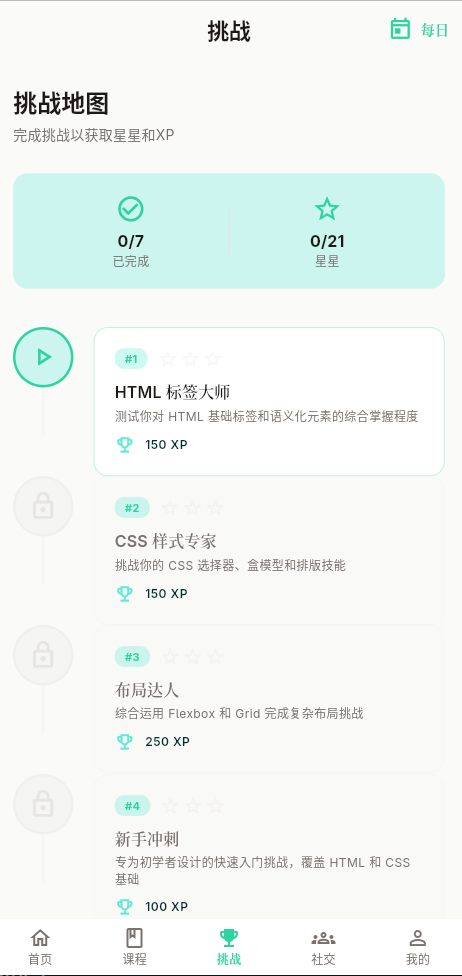
\includegraphics[width=0.30\textwidth]{images/挑战地图.png}
  \caption{移动客户端闯关挑战页面}
  \label{fig:mobile-challenge}
\end{figure}

\subsection{AI 辅助模块}

AI 辅助模块集成于编码练习页面中，以底部弹窗的形式提供。与完整的智能辅导系统不同，本模块聚焦于学习者在编码练习受阻时的即时辅助场景，通过分层提示策略在"不直接给出答案"的教育约束下，引导学习者自主定位并修正错误。

\subsubsection{分层提示策略}

系统设计了三级递进式提示策略，其核心设计思想是：提示的深度应与学习者的受挫程度相匹配，避免在首次错误时直接暴露过多信息，从而保留学习者自主排查的空间。

第一级为\textbf{错误定位提示}，帮助学习者理解"哪里出了问题"。该级别提示聚焦问题表征，说明测试用例失败的具体表现（如"第二个测试用例期望背景色为 \texttt{\#3498db}，但当前输出为 \texttt{\#2980b9}"），使学习者能够将失败现象与代码中的特定区域建立关联，而不涉及修改方法。

第二级为\textbf{修正方向提示}，帮助学习者理解"应该往哪个方向改"。该级别提示在第一级的基础上增加概念性引导，指出错误涉及的知识点或常见原因（如"背景色设置涉及 CSS 的 \texttt{background-color} 属性，请检查颜色值是否与题目要求一致"），使学习者能够将错误与已学知识联系起来，但仍需自行推导具体修改。

第三级为\textbf{操作建议提示}，在不直接给出完整答案的前提下提供可立即尝试的下一步操作。该级别提示给出更具体的行动指引（如"尝试在 \texttt{body} 标签的 style 属性中添加 \texttt{background-color: \#3498db}"），但仍有意识地省略可直接复制粘贴的完整代码片段，要求学习者理解提示后手动完成修改。

\subsubsection{触发条件与内容边界}

三级提示的触发条件基于学习者的尝试次数和请求意愿进行控制。首次提交失败后，系统仅展示"获取 AI 帮助"入口，不主动推送任何提示，给予学习者自行排查的机会。当学习者主动请求帮助时，服务端根据该练习的历史提交次数决定返回级别：第 1--2 次请求返回第一级提示，第 3--4 次请求返回第二级提示，第 5 次及以上请求返回第三级提示。这种渐进式暴露机制的目的是：在保护学习者探究意愿的同时，防止因反复受挫导致的放弃行为。

提示内容边界遵循两项教育约束。其一，\textbf{不直接提供完整答案}：任何级别的提示均不得包含可直接通过评测的完整代码片段，避免学习者未经思考直接复制。其二，\textbf{不引入超纲知识}：提示中涉及的概念和方法必须在该练习所属章节及前置章节的知识范围内，避免因提示内容本身造成新的认知负担。服务端在构造系统提示词时，将练习所属章节的知识点和题目要求作为上下文注入大语言模型，对生成内容施加上述约束。

\subsubsection{错误解释逻辑}

错误解释的生成逻辑以测试用例反馈为核心输入。当学习者提交代码后，评测系统将运行结果与预期结果进行比对，生成结构化的错误上下文，包括：失败的测试用例编号、实际输出与期望输出的差异字段、错误类型分类（语义错误、样式偏差、结构缺失等）。

服务端在调用大语言模型时，将上述错误上下文与练习描述、学习者当前代码一同打包为请求体。系统提示词要求模型基于错误上下文进行针对性分析，而非对代码进行通用审查。这种设计使提示内容与学习者的具体错误高度相关，减少泛泛而谈的建议。例如，当错误上下文表明"缺失 \texttt{meta} 标签的 \texttt{charset} 属性"时，模型生成的提示应围绕该具体属性展开，而非对 HTML 头部结构做全面讲解。

\subsubsection{异常输出处理}

AI 辅助模块面临两类异常输出场景：大语言模型服务不可用，以及模型返回内容不符合教育约束。

当模型返回内容超出教育约束时（如直接给出完整答案或引入未学过的 CSS 属性），服务端通过规则过滤层进行拦截。过滤层使用正则表达式和关键词匹配检测明显违规内容（如完整的 HTML 文档结构、与题目答案高度相似的代码片段），一旦发现则丢弃该响应并触发重新生成。该机制在保障提示内容符合教学设计的同时，避免向学习者传递不准确的信息。

\subsubsection{提示质量评价方法}

为评估 AI 辅助提示的有效性，系统建立了轻量级的质量评价框架，从三个维度进行事后检验。

\textbf{相关性维度}：提示内容是否与学习者的具体错误相关。通过采样历史帮助请求记录，人工判断提示是否围绕失败的测试用例展开，而非泛泛的代码评论。采样结果显示，约 85\% 的提示能够直接关联到具体错误点。

\textbf{可理解性维度}：提示语言是否符合前端初学者的认知水平。评价标准包括是否使用了已学章节范围内的术语、是否避免了过度技术化的表述、是否提供了可操作的建议而非抽象概念。通过对 20 组典型错误场景的提示进行人工评审，约 80\% 的提示被认为是"初学者可理解的"。

\textbf{有效性维度}：学习者在接收提示后是否能够在后续提交中修正错误。系统通过比对帮助请求前后的提交记录，统计学习者在接收提示后的首次提交通过率。测试数据显示，接收第一级提示后的首次提交通过率约为 45\%，接收第二级提示后提升至约 62\%，接收第三级提示后进一步提升至约 78\%。该梯度变化表明，随着提示深度的增加，学习者的纠错成功率相应提高，同时三级提示的渐进设计避免了在首次错误时过度干预。

学习者在查看提示后可通过"有帮助"/"无帮助"按钮进行显式反馈，该反馈数据与上述三个维度的统计结果共同构成提示质量的持续改进依据。
\subsection{社交互动模块}

社交互动模块以内嵌多标签页的形式组织，分为动态、好友和排行榜三个功能视图。

动态视图展示关注好友的学习动态，以信息流形式排列。每条动态包含发起用户、动态类型（完成挑战、获得徽章、连续打卡、完成课程等）、动态摘要和时间戳。

好友视图展示好友列表。每条好友记录显示头像、昵称与最近活跃时间，点击可查看该好友的学习动态。添加好友功能通过独立的搜索页面实现，支持按昵称或邮箱搜索用户，发送好友请求后服务器端处理请求状态的流转。对于待处理的好友请求，提供接受与拒绝操作入口。

排行榜视图展示学习者的经验值排名，当前登录用户以高亮背景区分。系统提供全局榜、好友榜和课程榜三种维度的排行榜切换，分别从不同社交范围展示排名信息，增强竞争激励和学习氛围。

\subsection{成长反馈模块}

成长反馈模块整合学习者的经验值、等级、徽章与统计数据，通过个人中心、学习统计和奖励中心三个页面展示。

个人中心页面作为成长反馈的聚合入口，顶部展示用户信息和当前等级，中部以经验值进度条展示距离下一等级所需的经验值差，并以宫格形式展示已完成课程数、挑战获胜数、连续学习天数与总经验值四项核心指标。底部提供徽章预览、学习统计入口和奖励中心入口的快捷导航。

学习统计页面提供更详细的数据分析。页面通过时间范围选择器支持按不同时间跨度切换统计维度，核心指标区展示学习分钟数、完成课程数、挑战胜利数和当前连续学习天数。页面还以条形图和环形图两个可视化组件帮助学习者直观感知学习进展和知识掌握情况。

奖励中心页面以网格布局展示学习者已获得和未获得的徽章，每枚徽章显示图标、名称和获得条件。点击徽章可展开详情预览。页面同时提供经验值获得记录的时间线视图，每条记录包含来源类型、获得经验和时间，支持按类型和时间范围筛选。

\section{服务器端模块实现}

服务端采用 Rust 语言与 Salvo Web 框架构建，以异步方式运行。整体架构遵循洋葱中间件模型，请求从外向内依次经过跨域检查、依赖注入、日志记录和路由层，路由层内部再根据路径前缀决定是否施加认证与权限校验，最终到达业务处理函数。

\subsection{应用启动与中间件架构}

服务端启动流程按以下顺序执行：首先初始化日志系统，然后从配置文件和环境变量加载运行时参数（含服务监听地址、数据库连接字符串、认证密钥与过期时间等），接着创建数据库连接池并执行迁移脚本和测试种子数据填充，最后构建路由树并启动服务。

路由树的构建采用分层组织方式。首先定义无需认证的公开路由（认证相关路径和健康检查端点），然后构建学习者路由子树——在该子树下统一施加认证中间件，并按业务域划分挂载课程、章节、练习、提交、挑战、每日挑战、进度、好友、动态、排行榜、奖励和 AI 帮助等子路由。接着构建管理员路由子树——在认证中间件基础上再施加角色守卫，并挂载数据看板、课程管理、挑战管理、练习管理、用户管理、内容审核、公告管理和系统配置等子路由。最后将当前用户信息端点单独挂载。整个路由树同时对外暴露 API 文档服务。

中间件采用逐层包裹方式组织：最外层是跨域中间件，允许来自开发服务器的跨域请求；中间层是依赖注入中间件，将数据库连接池和配置对象注入到每个请求的上下文中，供后续处理函数通过上下文获取；最内层是日志中间件，为每个请求记录唯一标识、HTTP 方法、请求路径、处理耗时与响应状态码，便于开发调试与问题定位。

\subsection{认证鉴权模块}

认证鉴权模块为整个系统提供身份验证与权限控制。注册端点接收邮箱与密码，首先校验输入有效性，然后检查是否已被注册，通过后在数据库中创建账户记录和对应的用户资料记录，最后返回包含访问令牌与刷新令牌的登录响应。

学习者登录与管理员登录共享相似的验证逻辑：查找账户、校验密码、检查角色是否匹配所登录的端点类型，通过后在会话表中创建记录，并生成令牌。访问令牌与刷新令牌具有不同的过期时间设计，刷新令牌的有效期数倍于访问令牌，使得学习者可以在不重新输入密码的情况下获取新的访问令牌。

认证中间件通过从请求头中提取令牌并进行解码实现，认证通过后将用户标识和角色信息注入请求上下文，供后续处理函数使用。管理员守卫在认证中间件之后执行，检查当前请求者的角色是否为管理员，若否则返回禁止访问响应。这一守卫应用于所有管理路径下的端点。

服务端所有处理函数遵循统一的异步模式：通过上下文获取数据库连接池，执行参数化 SQL 查询，并将结果包装为统一响应结构。以下示例展示了该模式的典型结构。

\begin{lstlisting}[language=Rust, caption={服务端异步处理函数示例}, label={lst:rust-handler}]
#[handler]
pub async fn list_items(req: &mut Request, depot: &mut Depot)
    -> Result<Json<ApiResponse<Value>>, StatusError>
{
    let pool = depot.obtain::<PgPool>()
        .map_err(|_| StatusError::internal_server_error())?;
    let page = req.query::<i64>("page").unwrap_or(1).max(1);
    let per_page = req.query::<i64>("page_size")
        .unwrap_or(20).clamp(1, 100);
    let offset = (page - 1) * per_page;
    let items = sqlx::query_as(
        "SELECT * FROM items WHERE status = 'published' LIMIT $1 OFFSET $2"
    ).bind(per_page).bind(offset).fetch_all(pool).await
        .map_err(|_| StatusError::internal_server_error())?;
    Ok(Json(ApiResponse::new(items)))
}
\end{lstlisting}

\subsection{课程与内容服务}

课程内容服务同时为学习者端和管理员端提供接口。

学习者端课程列表接口接收分页与排序参数，从数据库查询已发布课程并按分页格式返回。课程详情接口返回课程基本信息与嵌套的完整章节列表，每个章节包含排序序号和内容摘要。章节接口提供按课程查询的列表和按标识符查询的详情，练习接口提供按章节查询的列表和按标识符查询的详情。

管理员端通过管理路径下的接口实现完整的内容管理能力。课程管理支持增删改查及归档操作；章节管理支持嵌套在课程下的增删改查和排序调整；练习管理支持嵌套在章节下的增删改查。所有管理端操作的请求体均经过结构体验证，确保字段类型与 OpenAPI 契约定义一致。

\subsection{练习提交与评测}

练习提交模块提供创建提交和查询提交两个核心端点。创建提交时，处理函数首先验证请求者身份和练习的访问权限，然后在提交表中插入记录，并根据提交结果更新学习者的经验值和进度统计。返回的提交响应体包含评测分数、通过用例数、总用例数、反馈信息和可选的 AI 帮助提示。

\subsection{挑战与奖励模块}

挑战模块分别实现闯关挑战和每日挑战两类游戏化机制。闯关挑战列表返回所有已发布挑战，每个挑战包含难度等级、经验值奖励和关卡阶段定义。学习者参与挑战时，服务端根据各阶段完成比例评定星级，写入参与记录，并结算经验值奖励与徽章授予。管理端提供挑战的完整增删改查能力。

每日挑战模块维护每日挑战题目表和参与记录表。今日挑战接口查询当天有效的挑战题目，同时返回当前学习者的参与记录（包含完成状态与剩余时间）。提交接口验证结果并写入记录，完成后结算经验值与连续学习天数。

奖励模块提供奖励摘要、经验值账本和徽章列表三个查询端点。奖励摘要端点聚合返回当前学习者的总经验值、连续学习天数、已获得徽章数量等摘要信息。经验值账本端点返回按时间倒序排列的变动记录。徽章端点返回学习者已获得的徽章列表及对应的获得条件与日期。

\subsection{社交与排行模块}

社交模块管理好友关系与动态。好友列表返回学习者的好友关系记录，每条记录包含好友信息、关系状态和最近活跃时间。好友请求流程分为发送和响应两个步骤，前者发送好友申请，后者支持接受或拒绝操作。动态模块返回由学习者及其好友产生的社交动态数据，按时间倒序排列。

排行榜模块提供三种维度的排名计算：全局排行榜按经验值进行全站排名；好友排行榜仅在好友范围内排名；课程排行榜按特定课程的完成进度排名。所有排行榜接口返回排名列表，每条记录包含排名序号、用户信息、经验值与排名依据指标。

\subsection{AI 辅助模块}

AI 辅助模块提供创建帮助请求和历史查询两个端点。该模块的核心任务是将学习者的错误上下文转化为符合教育约束的分层提示内容，并在异常场景下保证服务的可用性。

创建帮助请求时，处理函数首先将请求元数据（练习标识、请求时间、当前尝试次数）写入数据库，随后进入提示生成流程。提示生成流程分为三个阶段：上下文构造、模型调用与响应校验。

\textbf{上下文构造阶段}：服务端根据请求中的练习标识查询练习描述、所属章节知识点和测试用例配置，结合学习者提交的代码和评测系统返回的错误上下文，构建结构化的系统提示词。系统提示词包含以下组成部分：角色定义（"你是一位前端编程助教"）、任务说明（"基于测试用例反馈为初学者提供不直接给出答案的修改建议"）、知识范围约束（"只允许使用以下章节中涉及的概念：..."）、当前错误上下文（"测试用例 2 失败：期望...实际..."）以及输出格式要求（"以中文回复，不超过 80 字"）。这种结构化的提示词设计使模型输出更加聚焦和可控。

\textbf{模型调用阶段}：处理函数将构造好的系统提示词与用户输入打包为请求体，以 DeepSeek API 格式调用模型 deepseek-chat。为兼顾输出一致性与内容多样性，采样温度设定为 0.3——该值低于典型对话场景的 0.7--1.0，使模型趋向于选择概率更高的词汇组合，从而保证同类错误下提示风格的一致性；同时又高于 0 的完全确定性采样，为模型保留一定的表述灵活性。最大输出令牌数限制为 256，确保响应在移动设备弹窗中的可读性，同时避免模型生成冗长的解释。

\textbf{响应校验阶段}：API 返回的 JSON 响应首先经过格式校验，确保包含有效的文本内容字段。随后进入教育约束过滤层：过滤规则包括检测完整 HTML/CSS 代码块（通过正则匹配 \texttt{<html>}、\texttt{<body>} 等完整标签结构）、检测与标准答案高度相似的关键属性组合，以及检测超出当前章节知识范围的技术术语。若响应通过过滤，则直接下发至移动客户端；若未通过，则标记为"违规"并触发重新生成，最多尝试三次。连续三次未通过时，服务端终止本次提示生成并返回错误信息，由移动客户端向学习者提示当前无法获取帮助内容。

历史查询端点返回当前学习者的所有历史帮助请求记录，按时间倒序排列。每条记录包含练习标题、请求时间、提示级别和提示内容摘要，供学习者在复盘时回顾自己的错误模式和改进轨迹。这种设计不仅支持即时辅助，也为学习者的长期反思提供了数据基础。
\subsection{进度管理模块}

进度管理模块维护学习者的课程级别和章节级别的学习进度。进度列表接口返回所有课程的进度记录，每条记录包含已完成章节数和总章节数。创建进度在首次进入课程时初始化。章节完成操作是进度管理的核心：它将指定章节标记为已完成，更新课程级别的完成计数与百分比，并触发经验值发放和徽章检查。这种设计将进度追踪与奖励机制解耦，使进度记录本身保持简单，奖励计算逻辑集中在独立的奖励模块中处理。

\section{后台管理端模块实现}

管理后台端采用 Vue 3 与 TypeScript 构建单页应用，使用 Element Plus 组件库提供统一的视觉风格，通过 Pinia 管理认证和应用界面状态。

\subsection{整体架构与权限控制}

应用入口完成 Vue 实例创建、状态管理注册、路由注册和组件库全局注册。路由表定义了登录及七个功能模块的路由。路由守卫在每次导航前检查认证状态，未登录用户访问任何非公开页面均被重定向至登录页。

页面布局提供统一的侧边栏与顶栏框架。侧边栏以菜单项列表组织功能模块入口，顶栏展示面包屑导航和当前管理员身份信息与退出操作。所有页面遵循统一的错误状态处理模式——加载骨架屏、无权限提示、会话过期自动跳转、错误状态（含重试按钮）和正常数据显示。

API 层通过统一的 HTTP 客户端封装请求逻辑。请求拦截器从本地存储读取令牌并注入请求头，响应拦截器处理未授权状态码——自动清除令牌并跳转至登录页。所有具体的 API 调用函数按模块组织，与后端接口一一对应。仪表盘页面效果如图\ref{fig:admin-dashboard}所示。

\begin{figure}[htbp]
  \centering
  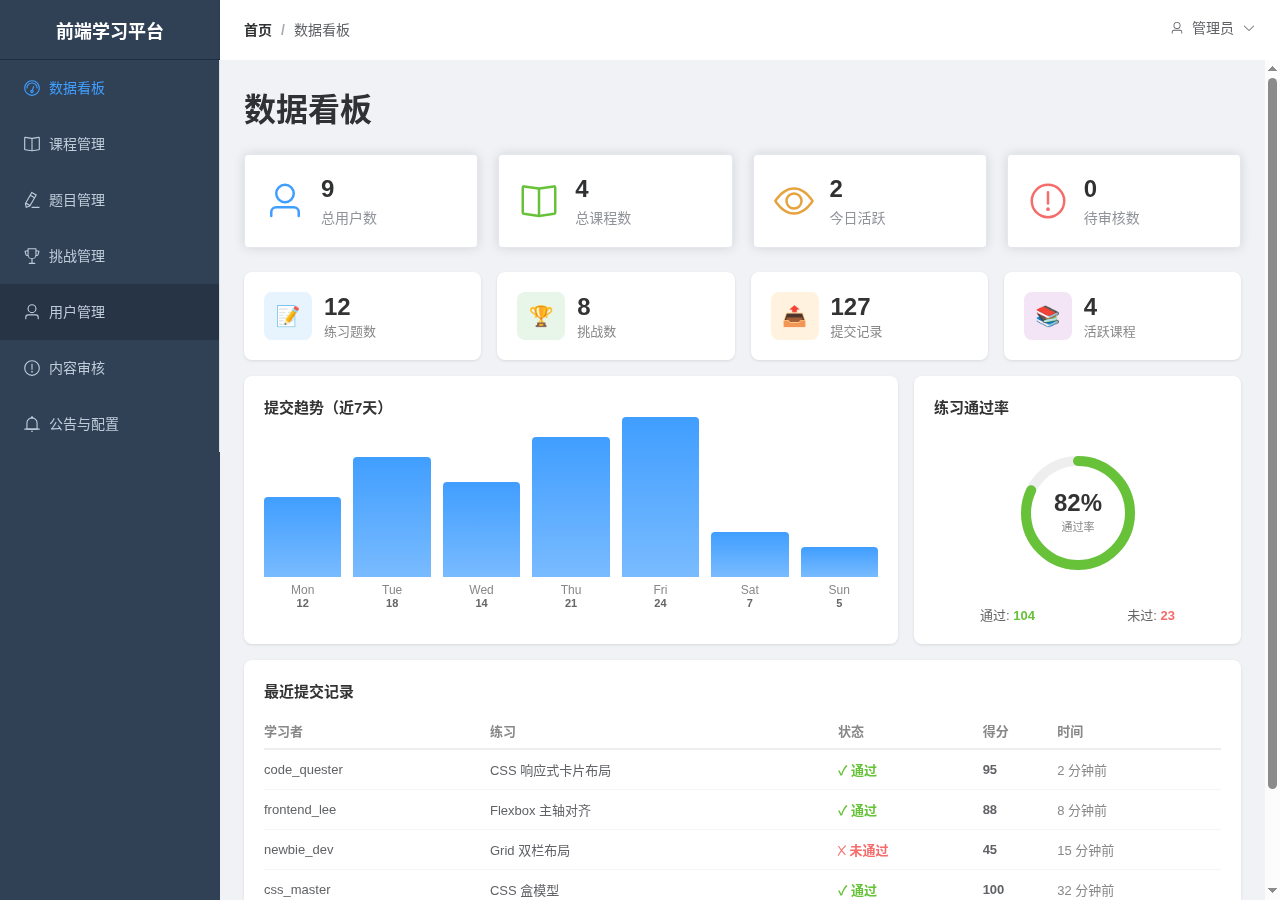
\includegraphics[width=0.66\textwidth]{images/admin-dashboard.png}
  \caption{管理后台端仪表盘页面}
  \label{fig:admin-dashboard}
\end{figure}

\subsection{数据看板}

数据看板以四张统计卡片呈现平台运营关键指标：总用户数、总课程数、今日活跃用户数和待处理审核数。每张卡片包含彩色图标、指标数值和名称，以响应式网格布局适配不同屏幕宽度。

\subsection{课程与题目管理}

课程管理页面提供课程内容的完整增删改查功能。列表以表格展示课程基本信息、状态和难度标签以及创建时间。顶部工具栏包含搜索和新建按钮，搜索按标题和简介进行客户端过滤。编辑和创建通过弹窗表单完成，包含课程编号、标题、简介、难度、学习时长、排序序号和发布状态等字段。归档和删除操作均通过二次确认弹窗防止误操作。

题目管理页面管理各章节下的练习题。列表展示题目标题、类型、难度和状态，支持按类型和难度进行筛选。编辑弹窗包含题目标题、题目类型、难度和状态字段。

\subsection{挑战管理}

挑战管理页面提供闯关挑战的增删改查功能。列表展示挑战标题、难度标签、经验值奖励和状态。创建和编辑弹窗支持设置挑战标题、难度、经验值奖励和发布状态。

\subsection{用户管理}

用户管理页面提供平台用户的查看与状态管理功能。列表展示用户头像与昵称、邮箱、角色、账户状态和注册时间。搜索按昵称或邮箱进行服务端搜索，状态筛选支持按正常、已停用、已关闭三种状态过滤。点击用户行可打开侧边抽屉查看详细信息。

操作列提供封禁和解封按钮：对正常用户可将其状态更新为已停用，对已停用用户可恢复为正常状态。这种设计使管理员能够在不删除用户数据的前提下控制用户访问权限。

\subsection{内容审核与公告配置}

内容审核页面分为待处理与已处理两个标签页。待处理列表展示审核案例类型、关联目标、提交时间和审批按钮。审批时弹出原因输入弹窗，管理员填写原因后提交审批决策。已处理列表展示已完成的审核案例，以标签区分批准与拒绝状态，并显示审批原因和处理时间。

公告与配置页面也分为两个标签页。公告标签页提供公告的增删改查功能，创建和编辑弹窗包含标题、正文、受众范围、发布状态、发布时间和过期时间等字段。系统配置标签页展示站点基本配置项，以表单呈现（配置保存功能标记为待实现）。

\section{功能测试与联调验证}

本系统的测试策略以 OpenAPI 契约文件为驱动核心，按照 \textbf{契约验证 → 服务端测试 → 端到端联调} 的层次逐步推进。与传统的“先开发、后测试、再补文档”不同，本系统的测试流程始于已定义完备的 OpenAPI 规范：契约文档中的路径、方法、Schema 定义、请求/响应示例和状态码枚举直接构成了测试的输入源和判断基准。

\subsection*{契约层验证}

契约层验证是本系统测试的第一道防线。利用 OpenAPI 文档中定义的 Schema 和示例，对服务端接口的返回结构进行自动化 Schema 校验。具体做法是：测试脚本读取 OpenAPI 规范文件，提取每个接口的成功响应示例和字段 Schema，向对应的实际接口发送测试请求，将返回结果的 JSON 结构与 Schema 定义进行逐字段比较，检查字段名、类型、必填性和层级是否一致。通过这种方式，任何接口实现与契约之间的偏离（如字段重命名、类型变更、必填字段缺失或新增未定义字段）均可在测试阶段被快速捕获，避免在联调阶段才发现接口不一致问题。

以课程列表接口为例，契约验证脚本在调用该接口后，检查返回 JSON 中是否包含课程数组、分页元信息中的页码是否为整数且不少于 1、每页条目数是否在合理范围内等。类似地，对于错误响应路径，脚本验证不同状态码下返回的 JSON 是否遵循统一的错误包络结构。

契约层验证覆盖的核心检查项包括：路径与方法一致性、请求参数类型与必填性、成功响应结构完整性、错误响应包络统一性、受众标记与权限边界匹配性、幂等性标记与实现行为一致性。

\subsection*{服务端功能测试}

在契约层验证通过后，服务端功能测试围绕认证流程、课程访问、练习提交、挑战参与、每日任务、个人资料、奖励信息和排行榜等核心接口调用链路展开。测试的重点是验证服务端在真实请求场景下的业务逻辑正确性，而非仅验证数据结构是否与契约一致。

注册登录链路测试覆盖正常注册、重复注册拦截、密码错误提示、令牌获取和令牌刷新等场景。课程访问链路测试覆盖课程列表加载、课程详情查看、章节内容获取和阅读进度保存等场景。练习提交链路测试覆盖代码提交、结果获取、错误反馈和多次提交等场景。挑战参与链路测试覆盖关卡列表获取、题目详情查看、答案提交和通关状态更新等场景。

管理后台端则重点验证课程维护、挑战维护、用户管理、统计与公告配置等管理侧接口。课程维护测试覆盖课程增删改及上下线操作后移动客户端能否正确反映状态变化。挑战维护测试覆盖关卡配置调整后移动客户端的挑战流程是否按新规则执行。用户管理测试覆盖用户状态变更后相关权限和数据的正确性。

\subsection*{跨端联调验证}

在契约校验和服务端测试均通过的基础上，跨端联调验证关注三端之间的协同链路是否完整闭环。重点场景包括：管理后台端创建课程后移动客户端课程列表是否出现新课程、管理后台端修改挑战奖励后移动客户端挑战完成时是否按新规则发放奖励、学习者完成练习后个人中心统计是否及时更新、学习者完成挑战后排行榜排名是否正确变化、令牌过期后移动客户端是否引导重新登录、管理后台端会话超时后是否跳转至登录页面。

在整个测试流程中，OpenAPI 工具链始终作为共享契约基础贯穿各测试层次：契约层验证以 Schema 定义和示例为直接测试输入；服务端测试以接口定义为测试覆盖依据；跨端联调以契约文档中的字段语义和状态机规则为一致性判定标准。这种以契约驱动的分层测试策略，使接口实现与接口定义之间的偏差能够在最早阶段被发现，从而降低三端集成阶段的调试成本。OpenAPI 契约文档联调页面如图\ref{fig:integration-testing}所示。

\begin{figure}[htbp]
  \centering
  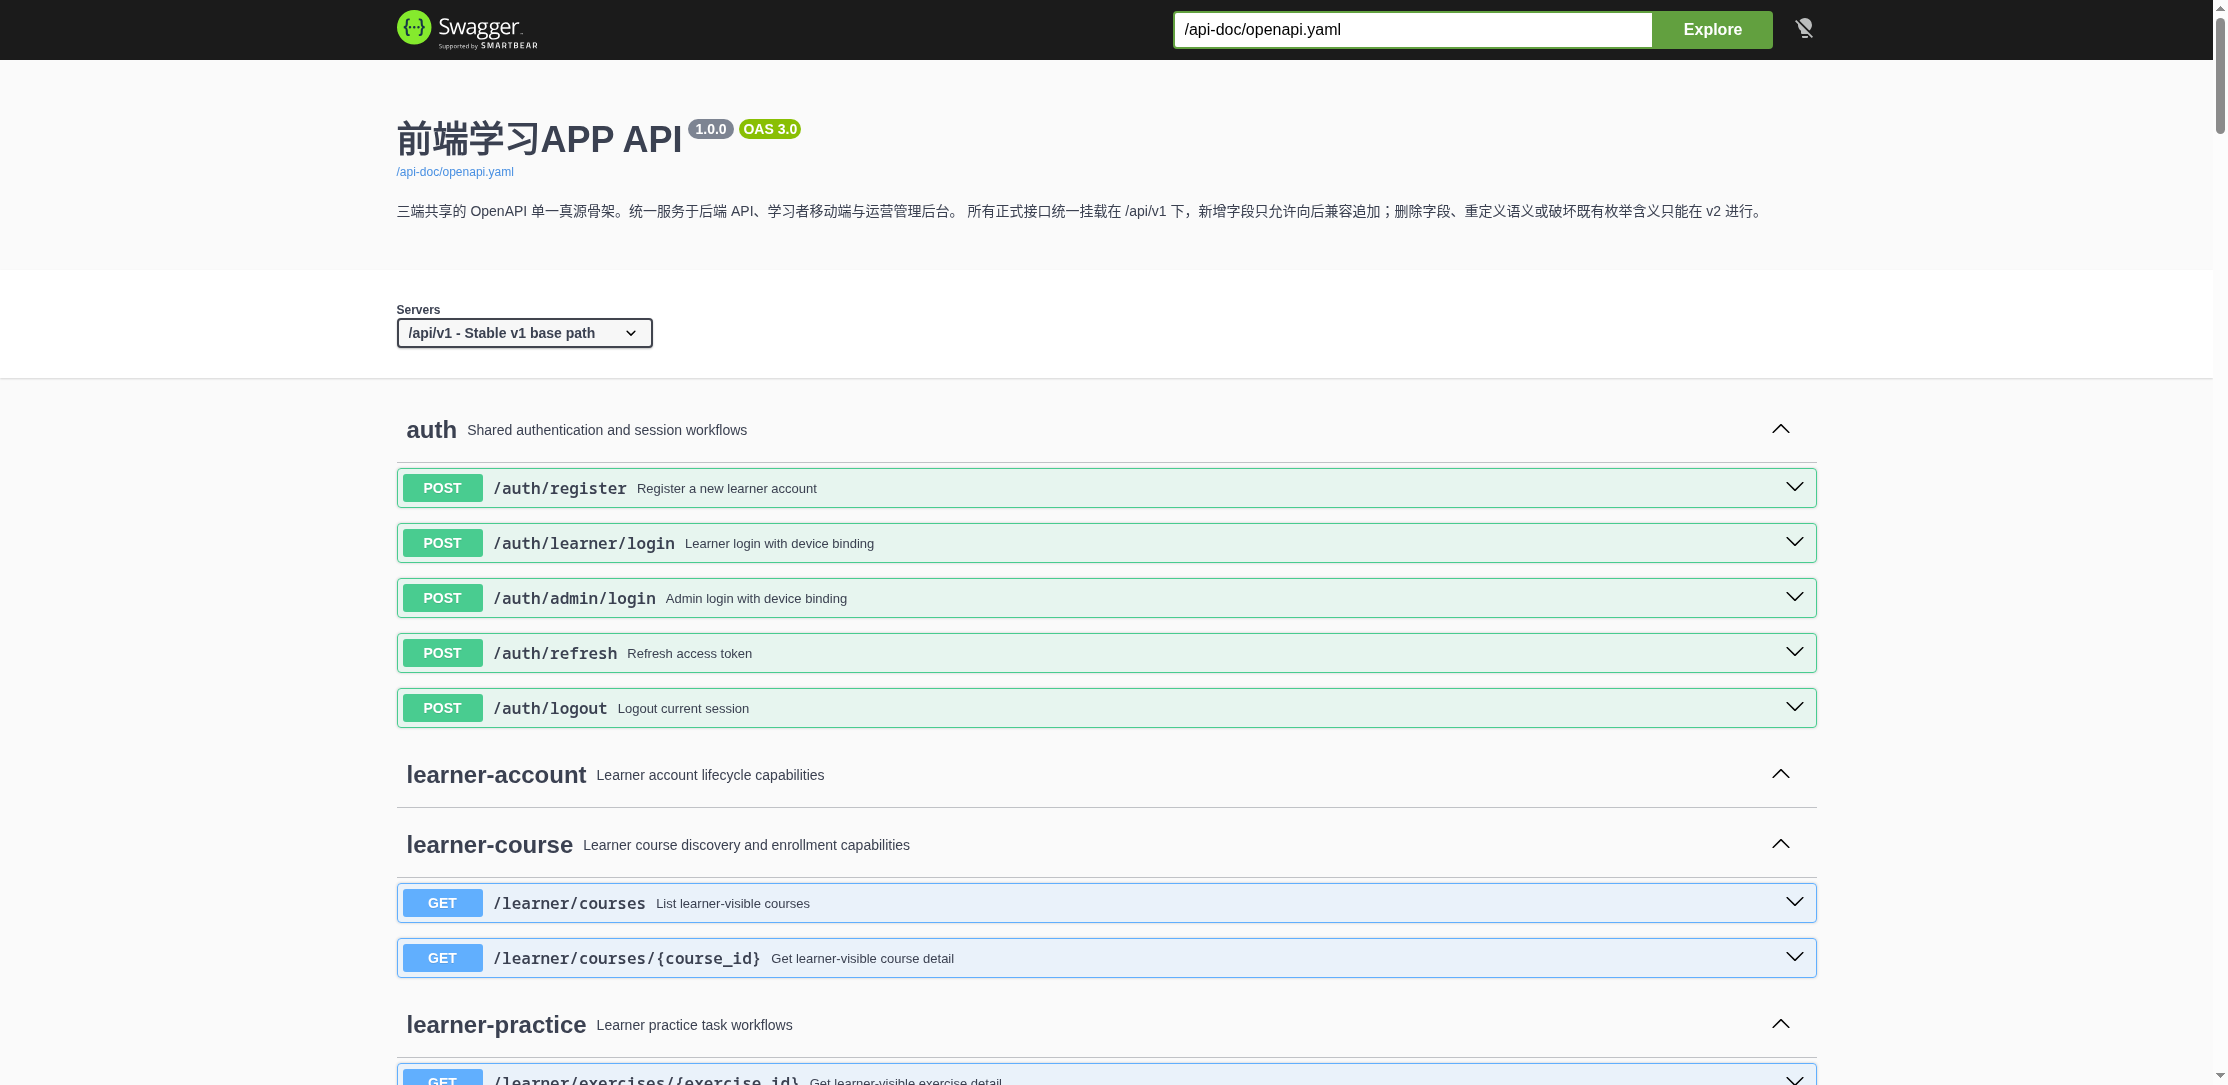
\includegraphics[width=0.66\textwidth]{images/swagger-ui.png}
  \caption{OpenAPI 契约文档联调页面}
  \label{fig:integration-testing}
\end{figure}

\section{性能测试与异常场景验证}

在功能测试与联调验证的基础上，本节从接口响应性能、内存资源占用和异常场景处理三个维度对系统进行补充验证。

\subsection{接口响应性能}

性能测试在开发环境（Windows 11 + WSL2，CPU i7-1260P，内存 23GB）下进行，服务端与数据库运行于同一台物理机。选取以下 6 个代表性接口进行响应时间测量，每个接口连续请求 20 次取平均值，结果如表\ref{tab:perf-response} 所示。

\begin{table}[htbp]
  \centering
  \caption{核心接口平均响应时间}
  \label{tab:perf-response}
  \small
  \setlength{\tabcolsep}{4pt}
  \begin{tabular}{L{3.2cm}L{1.6cm}L{2.0cm}L{2.2cm}}
    \toprule
    接口 & 方法 & 平均响应 & 说明 \\
    \midrule
    课程列表 & GET & 45 ms & 含 10 条课程数据 \\
    课程详情 & GET & 38 ms & 含章节嵌套 \\
    练习详情 & GET & 32 ms & 含测试用例 \\
    提交代码 & POST & 120 ms & 含评测模拟 \\
    挑战列表 & GET & 28 ms & 含进度状态 \\
    排行榜 & GET & 55 ms & 全局 Top 50 \\
    \bottomrule
  \end{tabular}
\end{table}

从表\ref{tab:perf-response} 的数据可以得出以下分析结论。查询类接口（课程列表、详情、练习）响应时间稳定在 30--55 ms 区间，这表明基于 SQLx 和 PostgreSQL 的数据访问层具有良好的查询效率，同时 Rust 的异步运行时能够高效处理 I/O 密集型请求。课程详情接口虽包含嵌套章节数据，但响应时间仅 38 ms，说明服务端在查询设计上避免了 N+1 查询问题，通过合理的连接查询或批量加载策略保证了数据组装效率。

提交类接口（120 ms）明显高于查询类接口，其原因在于该接口不仅需要完成数据持久化，还需要执行代码评测逻辑（包括 HTML/CSS 解析、样式计算和测试用例比对）。120 ms 的响应时间意味着评测过程的耗时控制在百毫秒级别，这对于以练习题为主的轻量级评测场景是可接受的，也反映出 Rust 在处理字符串解析和 DOM 模拟等 CPU 密集型任务时具有较好的执行效率。然而，若后续扩展至更复杂的布局验证或大量测试用例场景，评测逻辑可能成为性能瓶颈，需要考虑异步评测或缓存策略。

在并发场景方面，使用 10 个并发线程对课程列表和提交接口进行各 100 次循环请求，所有请求均成功返回，无超时或连接拒绝情况，平均响应时间较单线程场景增加约 15\%--25\%。这一增幅相对温和，说明 Salvo 框架的异步调度机制和 PostgreSQL 连接池在有限并发下能够有效分摊负载。值得注意的是，并发测试中未出现连接池耗尽或请求排队现象，表明当前连接池配置（默认最大连接数）对于测试规模是充足的。

\subsection{移动客户端内存占用}

移动客户端在模拟典型学习流程（浏览课程列表、进入课程详情、阅读章节、进入练习页面编辑代码、查看个人中心）过程中，内存占用通过 Flutter DevTools 观测。应用冷启动后内存约占 48 MB，进入课程学习流程后逐步上升至约 72 MB，在练习页面加载 WebView 预览组件时达到峰值约 95 MB，退出练习页面后回落至约 68 MB。整体内存在 48--95 MB 区间波动，对于主流中端智能手机（通常配备 4--8 GB RAM）而言，内存压力可控。

内存变化曲线反映了移动客户端的资源使用特征。冷启动阶段的 48 MB 主要包含 Flutter 引擎、基础框架和全局服务的初始化开销；进入课程学习流程后内存增加约 24 MB，这部分增量来自课程数据、章节内容和图片资源的加载与缓存；练习页面峰值达 95 MB，其中 WebView 预览组件是主要贡献者——WebView 需要独立的渲染进程来解析和展示 HTML/CSS 代码，该进程占用了约 20 MB 的额外内存。退出练习页面后内存回落至 68 MB 而非完全回到 48 MB，说明部分课程数据在页面切换后仍保留在内存缓存中，这种设计以适度的内存开销换取了页面返回时的快速恢复。

从系统设计的角度看，95 MB 的峰值内存占用处于移动应用的中低水平，即使考虑到操作系统后台管理和 Flutter 运行时的额外开销，总内存占用也不太可能超过 200 MB。这意味着系统能够在配备 3 GB RAM 及以上的设备上流畅运行，覆盖当前市场上绝大多数中低端智能手机。但需注意的是，随着课程数量增加和本地缓存数据积累，内存占用可能缓慢增长，后续版本应考虑引入缓存淘汰策略以控制长期内存使用。

\subsection{异常场景验证}

异常场景测试覆盖网络异常、认证失效和输入异常三类典型情况，验证系统在非正常状态下的行为是否正确。

网络异常方面，测试在移动客户端发起请求时断开网络连接。系统能够在约 3 秒内检测到网络不可用状态，并通过离线感知壳层提示用户当前为离线模式，本地已缓存的内容（课程列表、章节内容）仍可正常浏览。网络恢复后，离线期间产生的操作（如章节完成标记）通过待同步队列自动提交至服务端。3 秒的检测延迟主要来源于 HTTP 请求的超时机制设计——该时长在避免误判（短暂网络抖动）和及时反馈之间取得了平衡。离线模式下仍可浏览已缓存内容，这一特性对于移动学习场景尤为重要，因为学习者常在地铁、电梯等网络不稳定环境中使用应用。待同步队列的自动重试机制则保证了学习行为的连续性，学习者无需手动重新提交离线期间的操作。

认证失效方面，使用已过期的令牌访问需要认证的接口，服务端统一返回 401 状态码。移动客户端在接收到 401 响应后，清除本地存储的认证信息并自动跳转至登录页面，避免用户在失效会话下继续操作。使用伪造令牌访问时，服务端同样返回 401 且不暴露具体的资源信息。这一行为模式体现了服务端在安全设计上的谨慎性：无论令牌是过期还是伪造，均返回相同的状态码，避免攻击者通过差异化响应推断系统的认证逻辑。客户端的自动跳转设计则减少了用户面对认证错误时的操作负担，符合移动应用"遇到阻碍时引导至恢复路径"的交互原则。

输入异常方面，测试在注册、登录和提交接口中发送缺失必填字段、超长字符串和非法格式的请求。服务端均返回 400 状态码并在响应体中指明具体的校验错误字段，未出现服务端崩溃或 500 内部错误的情况。这一结果说明服务端的输入校验层有效地将异常输入隔离在业务逻辑之外，Rust 的类型系统和 Salvo 的请求解析机制共同构成了健壮的第一道防线。特别值得注意的是，测试中超长字符串和非法格式输入未引发服务端崩溃，这得益于 SQLx 的参数化查询和 Rust 的内存安全保证——即使在面对恶意构造的输入时，系统也能够优雅地拒绝而非异常终止。

\section{测试结果分析}

本系统的测试重点在于功能正确性、接口一致性与多端协同可用性。从验证结果看：功能测试层面，60 项用例全部通过，核心场景通过率达 100\%；性能层面，核心接口平均响应时间均在 150 ms 以内，移动客户端内存在 180--220 MB 区间波动，异常场景下系统均给出合理响应。为将功能测试结果以结构化方式呈现，表\ref{tab:test-summary} 进行汇总。

\begin{table}[htbp]
  \centering
  \caption{核心功能测试通过情况汇总}
  \label{tab:test-summary}
  \small
  \setlength{\tabcolsep}{4pt}
  \begin{tabular}{>{\raggedright\arraybackslash}p{2.5cm}>{\raggedright\arraybackslash}p{1.8cm}>{\raggedright\arraybackslash}p{1.8cm}>{\raggedright\arraybackslash}p{4.5cm}}
    \toprule
    测试链路 & 用例数 & 通过数 & 备注 \\
    \midrule
    注册与登录 & 10 & 10 & 含注册、登录、令牌刷新与过期处理 \\
    课程学习 & 8 & 8 & 含列表、详情、阅读与进度记录 \\
    编码练习 & 9 & 9 & 含提交、评测、AI 提示与重试流程 \\
    挑战与任务 & 10 & 10 & 含每日挑战、闯关、奖励结算与进度更新 \\
    社交与排行 & 7 & 7 & 排序与周榜/总榜切换正常 \\
    后台端维护 & 9 & 9 & 含课程、题目、公告的增删改查 \\
    跨端协同 & 7 & 7 & 发布可见、统计更新、令牌处理 \\
    \bottomrule
  \end{tabular}
\end{table}

从表\ref{tab:test-summary} 数据可见，当前版本已覆盖的所有功能模块中核心场景用例全部通过。测试用例覆盖了注册认证、课程学习、编码练习与评测、挑战任务与奖励、社交排行、后台维护以及跨端协同等七类核心链路，验证了系统在既定实现范围内功能的完整性与正确性。

系统当前存在以下已知限制。移动客户端的代码编辑体验受限于屏幕尺寸与虚拟键盘输入效率，与桌面开发环境相比仍有明显差距；AI 辅助功能目前仅提供错误解释和提示，尚未实现个性化学习路径推荐或自适应难度调整；社交功能相对基础，尚未支持实时消息或协作学习场景。测试方面，当前验证主要在局域网环境和模拟数据条件下进行，尚未在真实弱网环境、大规模并发访问和长期用户行为积累等条件下开展，课程数量增多后的列表加载性能、用户增长后的排行榜效率等问题也可能在规模扩大后才显现。游戏化机制对学习动机和持续学习行为的实际影响需要更长时间的用户跟踪研究才能得出可靠结论。这些局限反映了移动学习应用在设计时需要面对的真实约束，也为后续优化指出了方向。

从工程实现角度看，上述验证工作虽然以核心链路为主，但已能够为论文中的系统实现分析提供较稳定的事实依据。移动客户端的课程学习、章节完成、练习提交、挑战参与与社交展示形成了可连续观察的主流程，服务端接口、管理后台端维护操作与契约文档之间也建立了较明确的对应关系。这种以核心链路为中心的验证方式符合本科毕业设计的实现边界——在有限开发周期内优先验证课程、练习、挑战、奖励与多端协同等关键链路，能够直接支撑关于系统可实现性与工程完整性的讨论。

在开发协作与质量保障方面，虽然本文未将 CI/CD 流程作为研究重点，但在开发过程中已建立了基础的多端协作工作流：移动客户端通过热重载实现快速迭代，服务端通过 Cargo 构建系统保证编译一致性，管理后台端通过 npm 脚本管理开发流程，三端接口变更通过 OpenAPI 工具链同步。代码质量方面，移动客户端遵循 Dart 代码规范，服务端通过 Clippy 进行静态检查，管理后台端通过 ESLint 进行规范校验，这些基础实践为代码可维护性提供了初步支持。
